\chapter{Introduction}


\section{Brief Context for the Problem}

The Domain Name System (DNS), which converts domain names into IP addresses, is an element of the large network of digital communications. This system has an impact on the everyday digital interactions of each user, in addition to ensuring that the Internet runs smoothly. Unfortunately, this system is not resistant to abuse. Malicious actors use DNS domains for a variety of abusive, sometimes illegal activities, such as sending malware, phishing websites, and controlling botnets \cite{so2022}. These actions compromise the reliability and security of the Internet by posing serious risks to cybersecurity and user trust \cite{bayer2022}. Addressing this issue requires a robust response from DNS infrastructure providers, including registrars and registries, who play a role in the management of abuse complaints. Registries are organisations that manage top-level domains (TLDs) such as ".com " and ".net", and registrars are like a dealership for domain names.These entities have the authority to deactivate or deny the registration of DNS names if abuse is proven. Proactive measures are also considered, such as the refusal of registrations that could facilitate "typosquatting," and theoretically the regulation of permissible domain names to censor registration or renewal based on content. The effectiveness of these interventions could be improved by adopting a transparent approach to the measures implemented and the rationale behind such decisions. Although the publication of transparency reports can illuminate these practices, their issuance is rarely observed in the current landscape.

\begin{figure}[H]
    \centering
    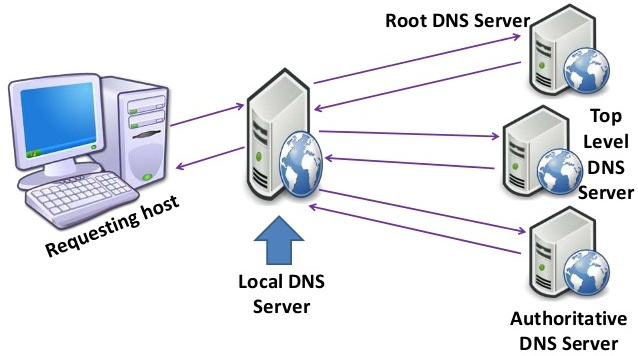
\includegraphics[width=0.5\linewidth]{introduction/dnsWork.jpg}
    \caption{How DNS works. Adapted from \cite{blanche2018understandingDNS}. }
    \label{fig:dnsIntro}
\end{figure}

\section{Motivation}

 The abuse of DNS for abusive, sometimes illegal activities, such as confusable domains and phishing, has raised questions about the integrity and security of the Internet. The severity and frequency of these concerns are highlighted in recent studies, such as the "Study on Domain Name System (DNS) Abuse: Technical Report" by Bayer et al. \cite{bayer2022}, highlighting the importance of more monitoring and mitigation tactics. Not only have significant cases of DNS abuse endangered user security, but they have also damaged the general trust in the digital economy. Users' trust in online services declines as they become more aware of these hazards, necessitating the implementation of mitigation measures to regain confidence and guarantee a secure online experience. According to Hesselman et al. \cite{hesselman2020}, the idea of a "responsible Internet" aims to increase confidence and sovereignty by improving network-level transparency and accountability. Furthermore, Mathew and Cheshire's \cite{mathew2016} study "Trust and Community in the Practice of Network Security" dives into the significance of trust connections and communities in cybersecurity, demonstrating the negative effects of DNS abuse on user trust.

\begin{figure}[H]
    \centering
    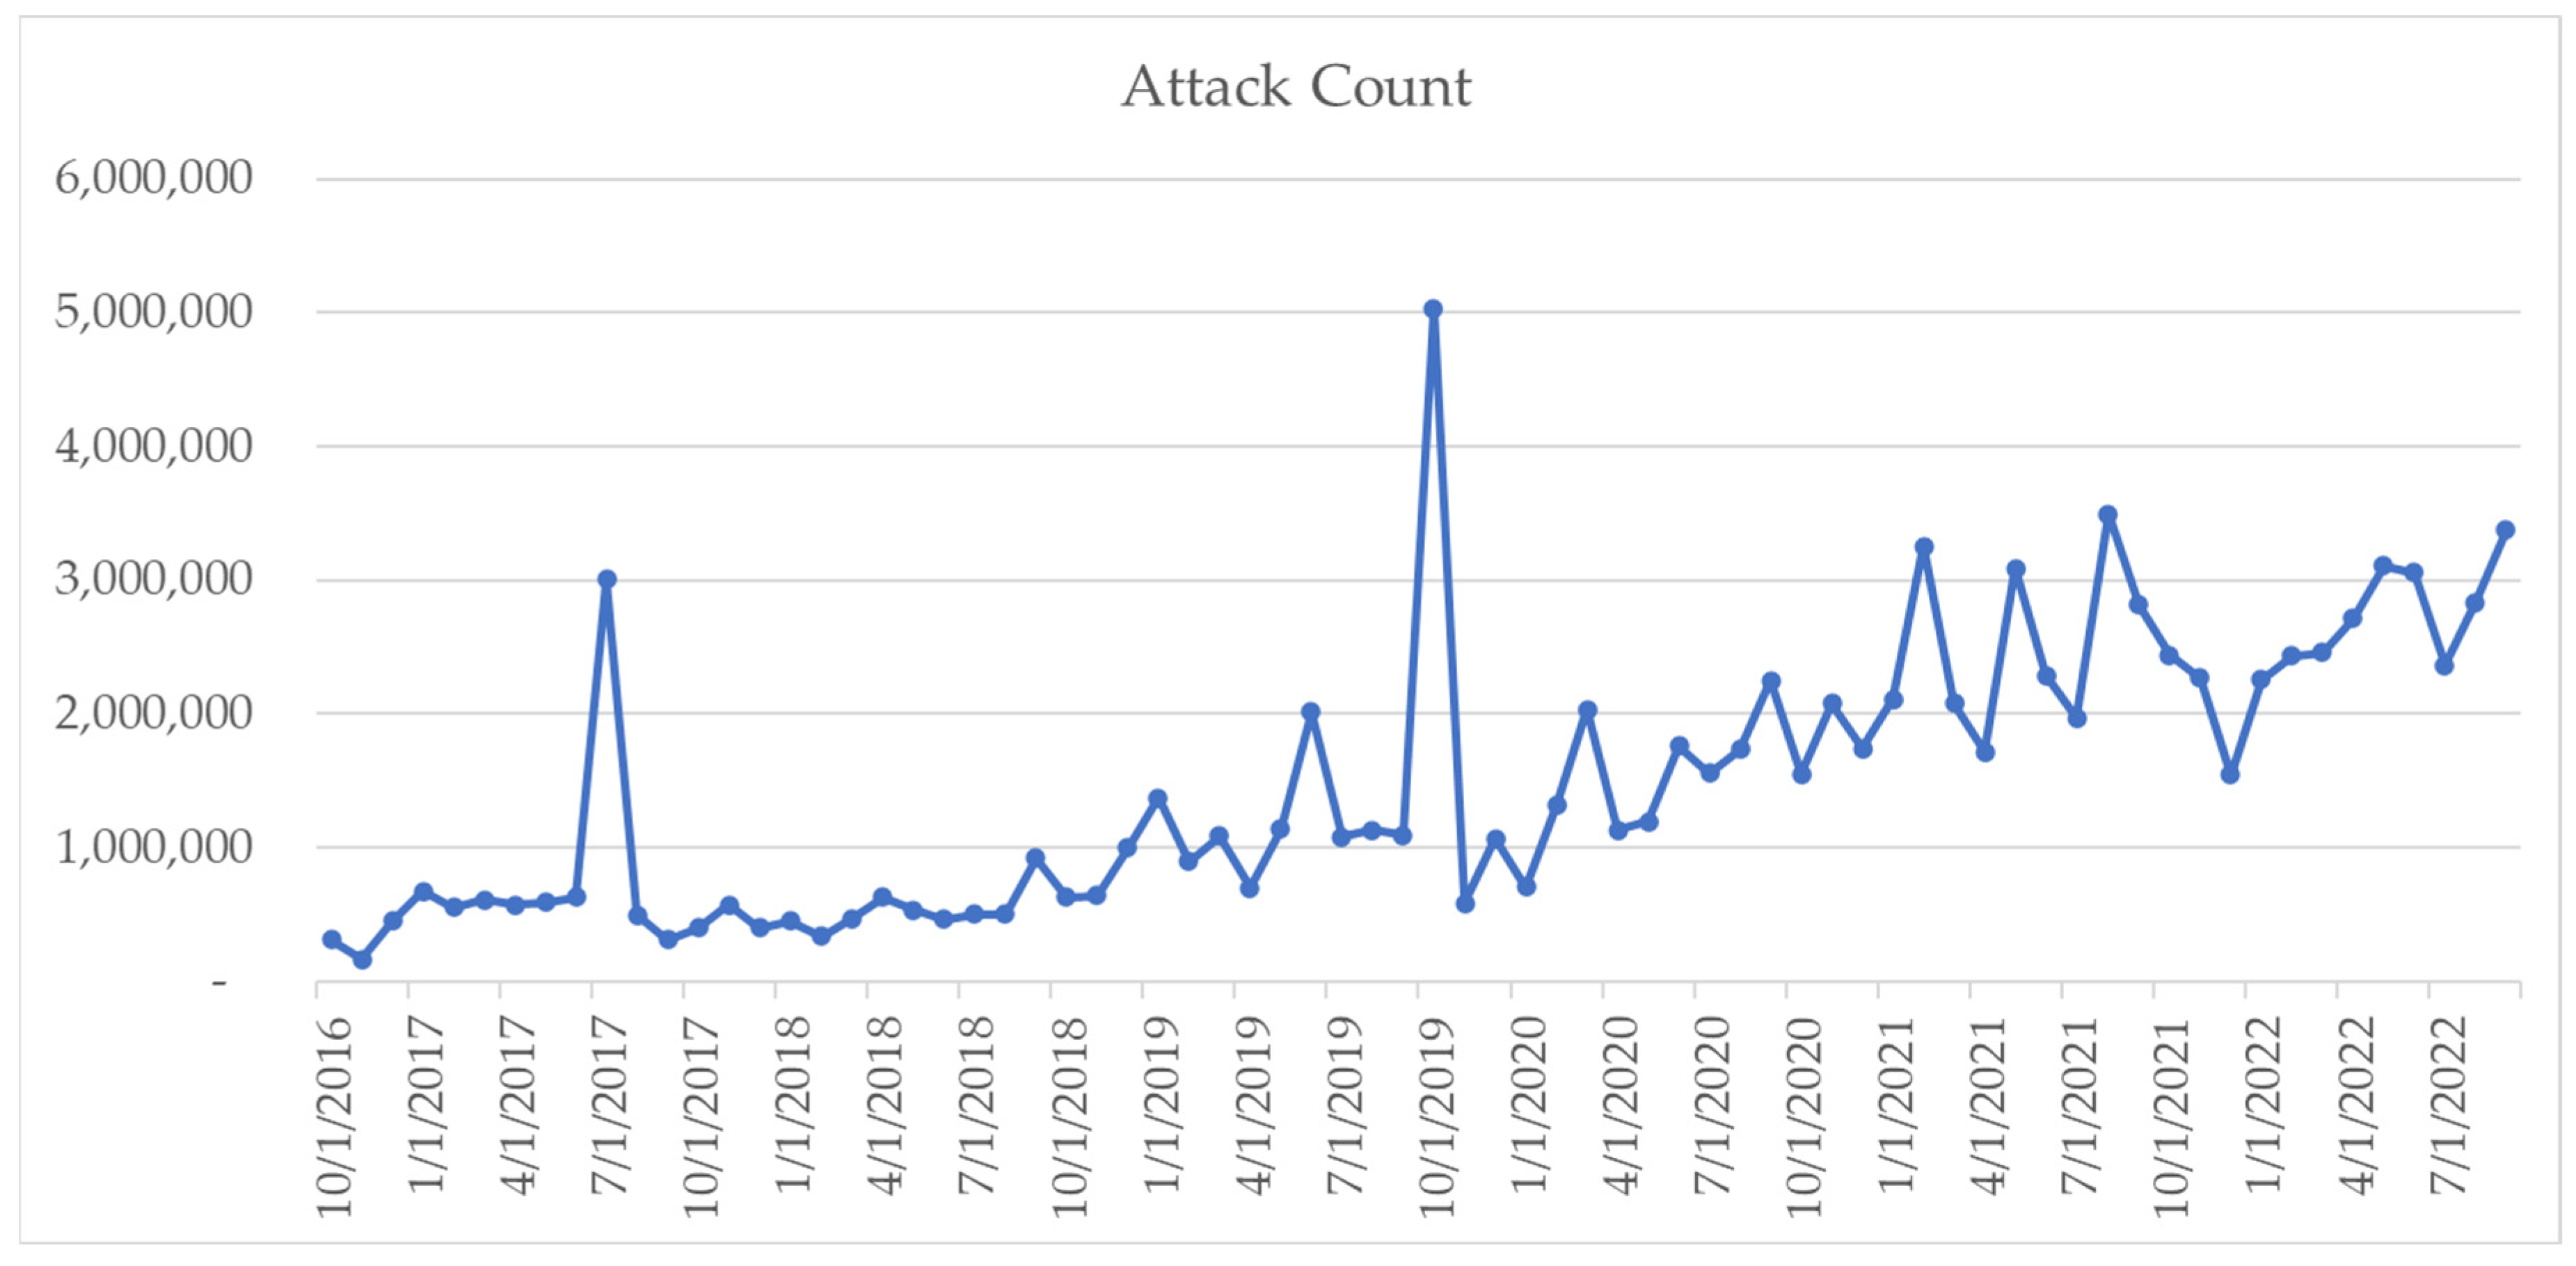
\includegraphics[width=0.9\linewidth]{introduction/maliciousActivity.png}
    \caption{ increase in DNS abuse incidents over time. Adapted from \cite{Rich2023Cyberpsychology}.}
    \label{fig:dnsintro2}
\end{figure}

Registries and registrars are leading the way in this issue, especially DNS infrastructure providers such as registrars and registries. However, their policies are probably clear and transparent to themselves, just not to outsiders. The continuous lack of confidence is made worse by the unclear way in which DNS abuse allegations are handled and the actions that follow. The importance of protecting the Internet and its reliability is recognised in relation to this issue \cite{cerf2022}. Furthermore, there are ethical and legal consequences to DNS abuse and how to mitigate it in addition to the technical ones. The goal of this project is to close this gap by investigating ways to improve the transparency of DNS abuse mitigation. This study aims to shine light on the present efforts and highlight the obstacles to greater transparency by assessing the current landscape of transparency reports and practices among DNS infrastructure providers. The ultimate objective is to provide a contribution to a system that promotes and enables more efficient and approachable transparency in the mitigation of DNS abuse.


\section{Research Question/Project \& Personal objective} 
\subsection{Research Question}

The primary research question for this project is: "How do the strategies and practices employed by registries, registrars, and other DNS infrastructure participants, as reflected in their transparency reports, contribute to mitigating DNS abuse, and what can these approaches teach us about developing best practices for transparency in handling DNS abuse complaints?". This question seeks to uncover the mechanisms, policies, and practices in place to mitigate DNS abuse and to what extent these efforts are transparent to the public and stakeholders.

\subsection{Project Objectives}

Assess handling of abuse complaints

\begin{itemize}
  \item Investigate the procedures and policies that DNS infrastructure providers have in place to handle abuse complaints.
  \item Document the types of DNS abuses that are most frequently reported and the response strategies used.
\end{itemize}

Assess Transparency Levels:

\begin{itemize}
  \item Analyse the current state of transparency in the actions taken by providers against DNS abuse.
  \item Identify what information is made public, how it is communicated, and the frequency of disclosure.
\end{itemize}

Evaluating Against Best Practices:

\begin{itemize}
  \item Compare the findings with best practices in the industry to identify areas of strength and opportunities for improvement.
  \item Highlight exemplary cases of transparency and effective abuse mitigation.
\end{itemize}

Develop recommendations :

\begin{itemize}
  \item Propose actionable recommendations for DNS infrastructure providers to improve their abuse handling and transparency.
  \item Suggest policy changes or initiatives that could standardise and improve practices in the industry.
  \item Feed into future work on ways in which best practices for transparency could be developed.
\end{itemize}

Contribute to stakeholder understanding: 

\begin{itemize}
  \item Provide insights that help stakeholders, including users, policymakers, and other providers, understand the landscape of DNS abuse handling and transparency.
  \item Offer a foundation for further research and discussion on improving DNS security and trust.
\end{itemize}

\section{Scope}	
The Scope of this project is to perform an examination of the transparency measures taken by registrars and registries to mitigate DNS abuse and to survey registries, registrars, and others involved in mitigating DNS abuse to collect and characterise the transparency reports currently available. In addition to examining current transparency reports to inform future work on ways in which best practices for transparency could be developed. To obtain opinions and insights on current procedures and difficulties, the project will interact with a variety of players in the DNS ecosystem, such as registries, registrars,and policy makers. As part of the research, a set of criteria will also be developed to assess how transparency affects the views of Internet users about trust and safety. It will, however, not include the development of brand-new transparency tools or systems; rather, it will concentrate on examining current procedures and making recommendations for improvements. The main goal of the research is to understand and improve transparency and its impacts. 

\begin{figure}[H]
    \centering
    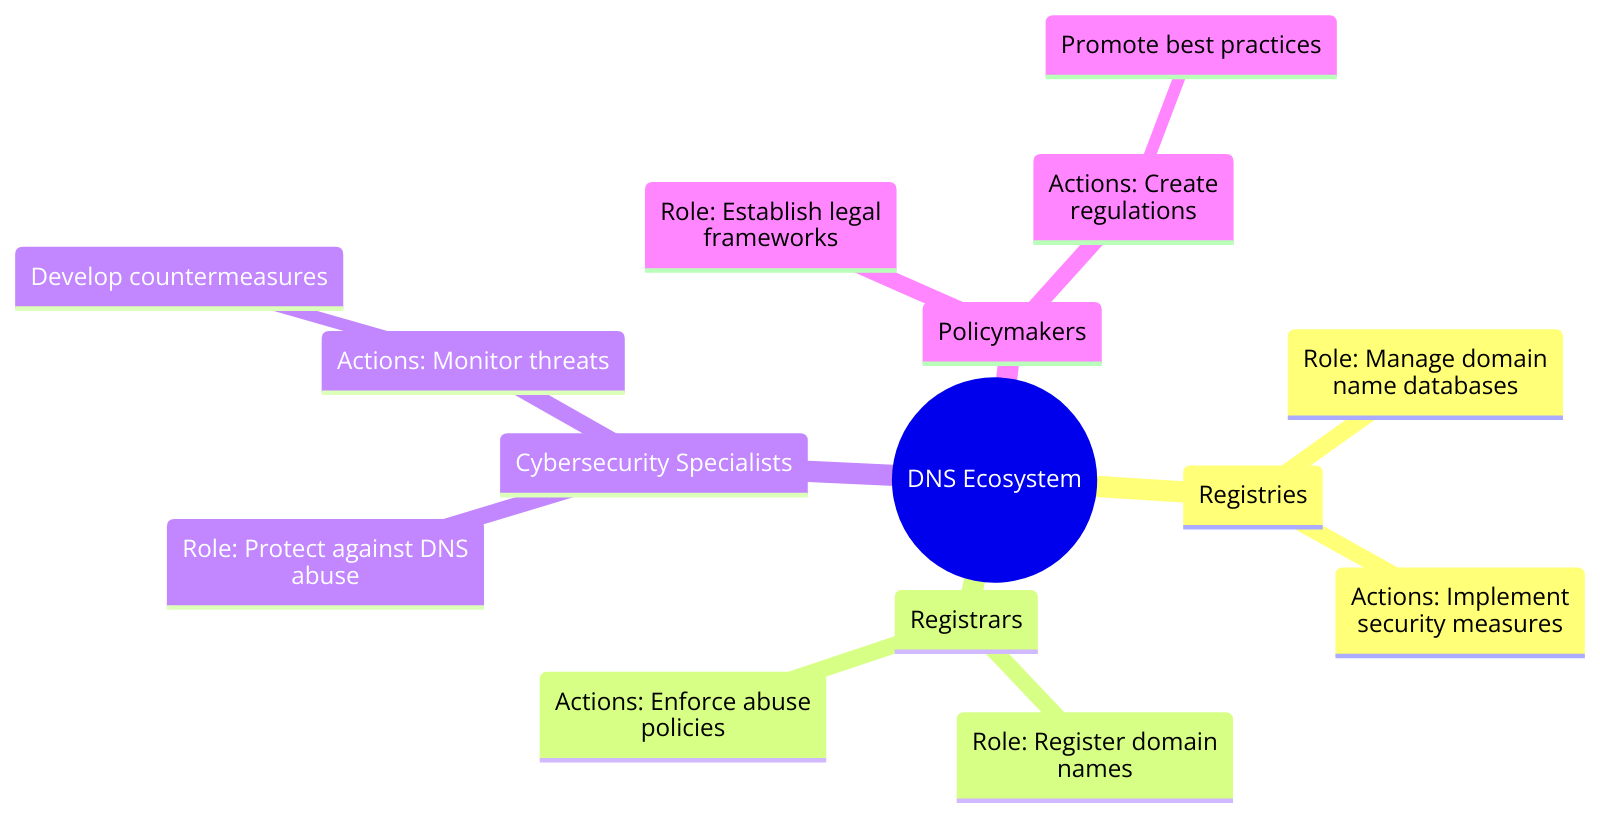
\includegraphics[width=\linewidth]{introduction/diagram (8).png}
    \caption{ DNS ecosystem.}
    \label{fig:dnsintrointro}
\end{figure}

\section{ Outline of the Project Work} 
The goal of this project, "DNS Abuse Transparency," is to better understand and increase the transparency of the efforts of the registrars and registries to mitigate DNS abuse. Research will first examine the different aspects of DNS abuse, such as popular forms like phishing, confusable domains, etc. and their broader consequences. 

Data gathering will be based on a questionnaire that will be distributed to a variety of DNS infrastructure providers and stakeholders throughout the world. The questionnaire attempts to shed light on current practices, the scope and efficacy of transparency measures, and the difficulties encountered in mitigating DNS abuse. At the same time, an examination of the transparency reports currently available from different sources will provide information on the transparency landscape, including the frequency, scope, and accessibility of these reports for users.

Critical evaluation of the handling of DNS abuse reports forms the core of the project. This involves looking at any proactive security measures that may be in place as well as the procedures for dealing with and preventing abusive domain registrations. After that, the research will change its focus to assessing how transparency affects user trust, provider reputation, and the general effectiveness of abuse mitigation techniques.

The project will discover and clarify best practices for transparency in the mitigation of DNS abuse, based on the data and insights obtained. The careful balance between security, privacy, and transparency will be taken into account by these best practices. The project will produce a series of practical suggestions for DNS infrastructure providers based on these findings, with the goal of improving transparency and, consequently, security and confidence in the digital ecosystem.

The project is designed to take place in a sequence of phases, each characterised by deliverables. A comprehensive timeline will guide the progress, guaranteeing an organised and exhaustive study of the subject. Upon completion, this project will have contributed a collection of recommendations and considerations for future study and policy creation in this area of Internet governance, in addition to offering a comprehensive understanding of the current state of DNS abuse transparency.

\section{Outline of the report}

This report offers a comprehensive account of the steps performed, decisions made, and research carried out during the project's development. The format of the report is as follows:

\textbf{Chapter 2 - Background }

This chapter examines the foundations of DNS , along with its significance, weaknesses, and several types of abuse. Observe the tactics and alliances used to combat DNS abuse, including the work of ICANN and the DNS Abuse Institute. The topic of DNS abuse is discussed along with its effects on users and potential risks in the future, with a focus on mitigation techniques and recommended practices.

\textbf{Chapter 3 -  State of the art }

This chapter critically analyses current strategies for DNS abuse mitigation and evaluates their effectiveness. Explores the complex relationship that exists between international governments and DNS, highlighting efforts to openness made by companies such as Google and Cloudflare. In addition to stressing the difficulties in striking a balance between user privacy and compliance requirements, the chapter emphasises the importance of DNS in internet governance. It investigates how various tactics are used and their effects on the larger online ecosystem through critical analysis.

\textbf{Chapter 4 -  Research methodology }

This chapter describes techniques to investigate DNS abuse and transparency from the infrastructure provider. The author goes on how the questionnaires were made, how the responses from stakeholders were analysed, and what kinds of DNS abuse were found. This chapter describes the methodology used to collect and examine data to understand DNS abuse reporting procedures and transparency policies.

\textbf{Chapter 5 -  Implementation }

This chapter involves the practical application, which involves findings from the project, especially the integration of the system, the back-end, the front-end implementations, and the technologies that comprise it. It includes how DNS data on abuse are visualised and the solution to the challenges during the implementation of the system. This part also includes testing and validation to ensure the success of the project.

\textbf{Chapter 6 -  Evaluation \& Discussion }

This chapter assesses how well the project addresses DNS abuse mitigation and improves transparency. Assesses the advantages of transparency in mitigating DNS abuse, as well as the security risks involved. The chapter also addresses the research limits and the degree to which the project's goals were achieved.

\textbf{Chapter 7 -  Conclusion }

This chapter summarises the project's results and recommendations to enhancing DNS abuse mitigation transparency. Consider the difficulties faced, the importance of continuous attempts to improve DNS security, and the possibilities for further study in this field. In conclusion, the importance of cooperation and transparency is emphasised in the fight against DNS abuse. 
